%\documentclass[proposal]{thesis} % use for a thesis proposal
\documentclass{thesis}

\usepackage{tikz}
\usetikzlibrary{shapes, arrows.meta, positioning, automata}

\subject{Exposé}
\title{Simulation of Distributed Majority Protocols}
\subtitle{Exploring Multi-Opinion Scenarios}
\author{Tom Groenwoldt}
\date{\today}
\location{Hamburg}
\supervisors{
Dr. Dominik Schallmoser\\ Institute for Data Engineering\\ TU Hamburg
}

\addbibresource{references.bib}


\begin{document}
\frontmatter
\maketitle
\tableofcontents
\mainmatter

\chapter{Exposé}

\section{Introduction}
The attainment of \textit{consensus} in a distributed system is a well-known and
researched problem. Distributed systems are a group of computers communicating
with each other to achieve a common goal. In terms of the consensus problem
a distributed system consists of \textit{n} agents. Individual agents may
hold exactly one of \textit{k} possible opinions. Consensus is reached by an
unanimous state, meaning every agent holds the same opinion. In order to reach
this state agents engage in mutual interaction and update their own opinion
based on a defined \textit{process} taking a set of agents as input.
\newline
The \textit{j-Majority} family defines a simple case of such a process. In
this configuration an agent selects \textit{j} other agents uniformly at random
(with replacement) and updates its own opinion to the opinion with the highest
majority from the selected set (ties are broken arbitrarily). Naturally, one
wants this to converge (reach consensus) in the fastest way possible. Now
the question is asked how the combination of different values for \textit{j},
\textit{k} and \textit{n} influence this goal.
\newline
Recent research has shown a hierarchy for majority protocols in the
case of \textit{bivalent} opinions. In particular it was proven that in the
family of \textit{j}-Majority (\textit{j} + 1)-Majority converges stochastically
faster when working in the \textit{gossip} and \textit{population model}.
The approach does not generalize for \textit{k} > 2 because it takes advantage
of the opinion distribution which is restricted to a binary opinion \cite{1}.
\newline
This thesis investigates whether a hierarchy between \textit{j}- and (\textit{j}
+ 1)-Majority regarding the convergence time exists for \textit{k} > 2 which
is an open question asked by Berenbrink et al. \cite{1}. For this purpose
we simulate the stated majority protocol for a dynamic number of agents and
opinions in the population and gossip model. The results are
then compared to the already researched case of \textit{k} = 2. Furthermore the
simulation is capable of defining a bias\footnote{The bias is the difference
between the numbers of agents holding different opinions} whose impact on the
convergence time is investigated as well. The purpose of this work is to lay
an empirically backed foundation for future work regarding convergence time in
majority protocols with multiple opinions.
\newline
In this exposé I present my planned methods of creating this simulation and
introduce helpful tools. Additionally I introduce relevant research references
to work with.

\section{Methodology}
Before starting with the simulation a broad overview about the topic of majority
protocols and their behavior should be gained and introduced to the reader.
The already researched hierarchy will then be explained in more detail. The
multi opinion scenario will be researched in general to make a justified guess
about the outcome of the simulation. In the next step the implementation steps
of the simulation will be documented as they form an important part of this
research and are crucial for understanding the outcome. After the successful
implementation of the software we are going to analyze the results and draw a
conclusion about the behavior of the protocol in regards to multiple opinions.
Additionally we plan to investigate the impact of a mutable bias for the initial
configuration.
\newline
The next subsections specify required features of the simulation software, the
tools to achieve this and a rough architecture.

\subsection{Requirements}
The software should be able to simulate the following things in the gossip- and
population model:

\begin{itemize}
\item Dynamic number of \textit{n} agents
\item Dynamic sample rate \textit{j} with \textit{j <= n}
\item Dynamic number of available opinions \textit{k}
\end{itemize}

It is important to note that a convergence to consensus can not be guaranteed
for every possible configuration. The simulation will therefore support a live
preview of the opinion distribution to inspect the progress while processing
and feature a maximum duration threshold which leads to abortion when passed.
\newline
The output should contain:

\begin{itemize}
\item Plots, similar to the empirical analysis in \cite{1}, for different values
of \textit{k}
\item Live view of opinion distribution
\end{itemize}

\subsection{Approach}
\textbf{Software.} The program will be modeled as a finite state machine on
the highest level of abstraction. First, the initial user defined configuration
is parsed. Then the simulation state will be entered. In this state the program
will act differently depending on the chosen model. Underlying data structures
should be used across those models. Every agent has the same implemented method
to execute the \textit{j}-Majority process function. This method takes a random
sample of \textit{j} elements from the agents set and adjusts the opinion of
the active agent as discussed above. The simulation is going to monitor the
current opinion distribution and will stop after reaching consensus. We will also
consider to add a feature flag for execution of multiple lined up simulations.
\newline
The duration of the time to attain consensus is logged by creating a timestamp
at the start and at the end. The corresponding difference as well as all
input parameters \textit{j}, \textit{n} and \textit{k} set by the user
are stored inside a CSV\footnote{\url{https://en.wikipedia.org/wiki/Comma-
separated\_values}} file. The format is valid for the input of the \LaTeX
package \textit{pgfplots}.

\begin{figure}[H]
\centering
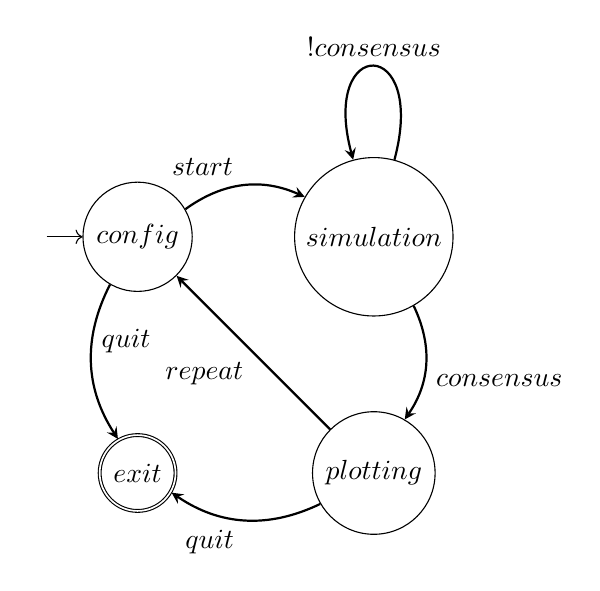
\begin{tikzpicture} [
	node distance = 3cm, 
    on grid, 
    auto,
    every loop/.style={stealth-}]
 
% State q0 
\node (q0) [state, 
    initial, 
    initial text = {}] {$config$};
 
% State q1    
\node (q1) [state,
    right = of q0] {$simulation$};
 
\node (q2) [state,
    below = of q1] {$plotting$};

\node (q3) [state,
    accepting, 
    below = of q0] {$exit$};

% Arrows
\path [-stealth, thick]
    (q0) edge[bend left] node {$start$}   (q1)
    (q0) edge[bend right] node {$quit$}   (q3)
    (q2) edge node {$repeat$}   (q0)
    (q1) edge[bend left] node {$consensus$}   (q2)
    (q1) edge [loop above]  node {$!consensus$}()
    (q2) edge[bend left] node {$quit$}   (q3);
\end{tikzpicture}
\caption{Automaton concept}
\end{figure}

\begin{figure}[H]
\centering
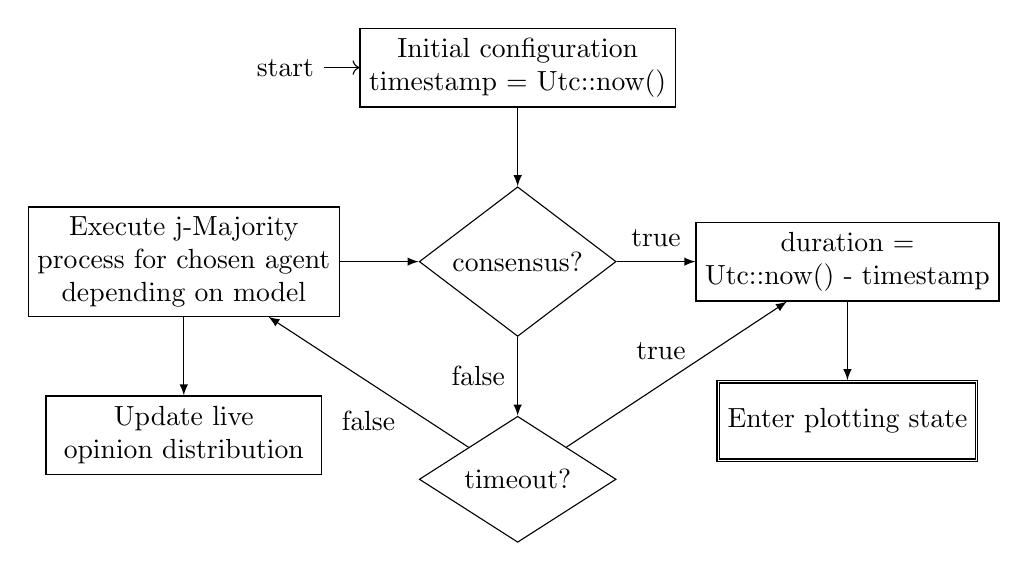
\begin{tikzpicture}

\node[draw,
    initial,
    align=center,
    minimum width=1cm,
    minimum height=1cm
] (block0) {Initial configuration\\timestamp = Utc::now() };
 
\node[draw,
    diamond,
    below=of block0,
    minimum width=2.5cm,
    inner sep=0] (block1) {consensus?};
 
\node[draw,
    diamond,
    below=of block1,
    minimum width=2.5cm,
    inner sep=0] (block5) {timeout?};

\node[draw,
    right=of block1,
    align=center,
    minimum width=3.5cm,
    minimum height=1cm
] (block2) {duration = \\ Utc::now() - timestamp};
 
\node[draw,
    left=of block1,
    minimum width=3.5cm,
    align=center,
    minimum height=1cm
] (block3) {Execute j-Majority\\process for chosen agent\\depending on model};

\node[draw,
    below=of block3,
    align=center,
    minimum width=3.5cm,
    minimum height=1cm
] (block6) {Update live\\opinion distribution};

% Return block
\node[draw,
    accepting,
    below=of block2,
    minimum width=2.5cm,
    minimum height=1cm,] (block4) {Enter plotting state};
 
% Arrows
\draw[-latex] (block0) edge (block1);
\draw[-latex] (block3) edge (block1);
\draw[-latex] (block2) edge (block4);
\draw[-latex] (block3) edge (block6);

\draw[-latex] (block1) edge node[yshift=0.3cm] {true} (block2);
\draw[-latex] (block5) edge node[yshift=0.3cm, xshift=-0.2cm] {true} (block2);
\draw[-latex] (block1) edge node[xshift=-0.5cm] {false} (block5);
\draw[-latex] (block5) edge node[yshift=-0.5cm] {false} (block3);

\end{tikzpicture}

\caption{Simulation concept}
\end{figure}

\textbf{Comparison and Analysis.} The output data is plotted the same way done
in the empirical analysis of \cite{1} and then compared to the proven hierarchy
for the case of \textit{k} = 2. We iterate over \textit{k} and for each
\textit{k} multiple biases are simulated. The impact of \textit{k} and those
biases is further analysed.

\subsection{Tooling}
The simulation will be written in Rust\footnote{\url{https://www.rust-
lang.org/}} as it is quite fast\footnote{\url{https://kornel.ski/rust-c-
speed}} and I already have experience with it. The Rust ecosystem consists of
many \textit{crates} (which are libraries) for all necessary requirements. The
simulation will feature a simple frontend for configuration and live view.
\vspace{10pt}
\newline
This is a list of promising crates and frameworks, all written in Rust. Please
note that this list is just a provisionally suggestion.

\begin{itemize}
\item \textbf{rand} - Utilities to generate random numbers, to
convert them to useful types and distributions, and some randomness-related
algorithms.
\item \textbf{chrono} - Proficient time logging
\item \textbf{Dioxus} - Portable, performant, and ergonomic framework for
building cross-platform user interfaces
\item \textbf{umya\_spreadsheet} - Write data to CSV file
\end{itemize}

The source code will be available via my GitHub account\footnote{\url{https://
github.com/tomgroenwoldt}}.

\section{Relevant references}
Of course, the already mentioned paper of Berenbrink et al. \cite{1} forms
a direct dependency for this thesis. It motivates this approach and allows
a comparison to the case of binary opinions and is therefore included in the
reference list.
\newline
The case researched in this thesis is not always guaranteed to converge,
that is why it is a good idea to gain knowledge about the case of divergence. A
promising paper could be \cite{becchetti2015stabilizing}. The goal of this paper
is the stabilization of the \textit{3}-Majority protocol with multiple opinions.
\newline
The paper \cite{becchetti2015simple} researched a bound for the initial bias to
achieve \textit{plurality consensus}\footnote{Plurality consensus is achieved
by having all nodes agree on the initial plurality} for \textit{k} > 2 possible
opinions. This will help to justify the divergence of some simulated cases.
\printbibliography

\end{document}
